\documentclass[11pt,a4paper]{article}
\usepackage[utf8]{inputenc}
\usepackage[italian]{babel}
\usepackage{amsmath}
\usepackage{amsfonts}
\usepackage{amssymb}
\usepackage{array}
\usepackage{graphicx}
\usepackage{multirow}
\usepackage{color,colortbl}
\usepackage{hyperref}
\hypersetup{colorlinks,urlcolor=blue,linkcolor=black}
\usepackage{fancyhdr}
\usepackage{tabularx}
\usepackage{enumitem}
\usepackage[left=2cm,right=2cm,top=2cm,bottom=3cm]{geometry}
\usepackage{ltablex}
\usepackage{listings}

\usepackage{lastpage}
\usepackage{titlesec}
\usepackage{xcolor}

\definecolor{lightgray}{rgb}{.9,.9,.9}
\definecolor{darkgray}{rgb}{.4,.4,.4}
\definecolor{purple}{rgb}{0.65, 0.12, 0.82}

\lstdefinelanguage{JavaScript}{
	keywords={typeof, new, true, false, catch, function, return, null, catch, switch, var, if, in, while, do, else, case, break},
	keywordstyle=\color{blue}\bfseries,
	ndkeywords={class, export, boolean, throw, implements, import, this},
	ndkeywordstyle=\color{darkgray}\bfseries,
	identifierstyle=\color{black},
	sensitive=false,
	comment=[l]{//},
	morecomment=[s]{/*}{*/},
	commentstyle=\color{purple}\ttfamily,
	stringstyle=\color{red}\ttfamily,
	morestring=[b]',
	morestring=[b]"
}

\lstset{
	language=JavaScript,
	backgroundcolor=\color{lightgray},
	extendedchars=true,
	basicstyle=\footnotesize\ttfamily,
	showstringspaces=false,
	showspaces=false,
	numbers=left,
	numberstyle=\footnotesize,
	numbersep=9pt,
	tabsize=2,
	breaklines=true,
	showtabs=false,
	captionpos=b
}

\renewcommand{\lstlistingname}{Esempio}% Listing -> Algorithm
\renewcommand{\lstlistlistingname}{Elenco degli Esempi}% List of Listings -> List of Algorithms

\pagestyle{fancy}
\fancyhf{}
\lhead{
\includegraphics[scale=0.07]{images/logo.png}}

\renewcommand {\footrulewidth}{0.2mm}
\lfoot {Analisi dei requisiti}
\rfoot{Pagina \thepage\ di \pageref{LastPage}}


\usepackage{appendix}
\usepackage{longtable}

\definecolor{LightBlue}{rgb}{0,0,0.5}
\definecolor{Gray}{gray}{0.8}
\definecolor{LightGray}{gray}{0.9}

\setcounter{tocdepth}{4}
\setcounter{secnumdepth}{4}

\titlespacing*{\subsection}{0pt}{8ex plus 1ex minus .2ex}{2.3ex plus .2ex}
\titlespacing*{\subsubsection}{0pt}{8ex plus 1ex minus .2ex}{2.3ex plus .2ex}

\begin{document}
	\begin{titlepage}
  \centering
	\scshape
	
	\vspace*{2cm}
	
\includegraphics[scale=0.7]{images/logo.png}
	\rule{\linewidth}{0.2mm}\\[0.37cm]
	{\Huge Piano di progetto}\\
	\rule{\linewidth}{0.2mm}\\[1cm]
	{\LARGE\bfseries Progetto Colletta - Gruppo OttoBit}\\[1cm]
	
	
	
	\begin{tabular}{>{\columncolor{Gray}}r | >{\normalfont}l}
		\rowcolor{LightBlue}		
		\multicolumn{2}{c}{\color{white}{Informazioni sul documento}}\\
		Versione & 1.0.0 \\
		Redazione & Benedetto Cosentino\\
							& Enrico Marcato\\
 		Verifica & Giovanni Peron\\
 		Responsabile & Benedetto Cosentino\\
 		Uso & Esterno\\
 																 		& Prof. Tullio Vardanega\\
 																		& Prof. Riccardo Cardin\\
 		\multirow[t]{-3}{*}{Destinatari}	& MIVOQ s.r.l\\
 		\hline
	\end{tabular}
\end{titlepage}
	{\def\arraystretch{2}\tabcolsep=10pt
	\newpage
	\section*{\centering Registro delle modifiche}
	\begin{tabularx}{\textwidth}{ c | c | c | c | X }
		\rowcolor{LightBlue}
		\color{white}\bfseries Versione & \color{white}\bfseries Data & \color{white}\bfseries Autore & \color{white}\bfseries Ruolo & \multicolumn{1}{c}{\color{white}\bfseries Descrizione}\\[0.25cm]
		0.0.1 & 2019-03-19 & Benedetto Cosentino & Progettista & creazione documento\\ \hline
		
	\end{tabularx}
	\newpage
	\tableofcontents
	\newpage
	\listoffigures
	\newpage
	\listoftables
	\newpage
	\lstlistoflistings
	\newpage	

	\section{Introduzione}
	\subsection{Scopo del documento}
	Il documento ha lo scopo di definire la pianificazione del progetto ``Colletta: piattaforma raccolta dati di analisi di testo" proposto da MIVOQ S.r.l. per il gruppo OttoBit. Il documento viene aggiornato durante le attività di incremento che lo riguardano ogniqualvolta è necessario. Al suo interno presenta:
	\begin{itemize}
		\item un'analisi dei rischi in cui è possibile incorrere;
		\item una breve analisi sul modello di sviluppo scelto;
		\item la pianificazione dei tempi e delle attività;
		\item l'assegnazione delle attività pianificate ai membri del team;
		\item una stima preventiva delle risorse;
		\item la rendicontazione delle risorse impiegate.
	\end{itemize}

\subsection{Scopo del prodotto}
	Il prodotto richiesto dalla proponente è una piattaforma che permetta la raccolta di dati in modo implicito tramite la risoluzione di esercizi. Tali dati devono essere utilizzati per addestrare un software di apprendimento automatico$^*$ già esistente che, a sua volta, deve essere in grado di fornire una soluzione agli esercizi proposti. L'obiettivo del prodotto potrà essere raggiunto tramite l'impiego di un database$^*$ che garantisca la permanenza dei dati, il software di apprendimento automatico e un'interfaccia (web o di un'applicazione mobile) che permetta l'interazione con gli utenti.

\subsection{Glossario}
	All'interno del documento è possibile trovare termini ambigui: in tal caso, tali termini possono essere trovati nel Glossario insieme alla relativa spiegazione. I termini del glossario vengono indicati con un * in apice.
	
\subsection{Riferimenti}
	\subsubsection{Normativi}
		\begin{itemize}
			\item \textit{NormeDiProgetto\_v2.0.0;}
			\item Capitolato d'appalto C2: Colletta\footnote{\url{https://www.math.unipd.it/~tullio/IS-1/2018/Progetto/C2.pdf}}
			\item Regolamento organigramma\footnote{\url{https://www.math.unipd.it/~tullio/IS-1/2018/Progetto/RO.html}}
		\end{itemize}
	\subsubsection{Informativi}
		\begin{itemize}
			\item ISO/IEC 12207:1995$^*$ \footnote{\url{https://en.wikipedia.org/wiki/ISO/IEC_12207}}
			\item ``Il ciclo di vita del software", slide del corso ``Ingegneria del software" \footnote{\url{https://www.math.unipd.it/~tullio/IS-1/2018/Dispense/L05.pdf}}
			\item ``Gestione di progetto", slide del corso ``Ingegneria del software" \footnote{\url{https://www.math.unipd.it/~tullio/IS-1/2018/Dispense/L06.pdf}}
		\end{itemize}

\subsection{Scadenze scelte}
	Il gruppo OttoBit ha scelto di rispettare le seguenti scadenze:
	\begin{enumerate}
		\item Revisione dei Requisiti: 2019-01-21;
		\item Revisione di Progettazione: 2019-03-15;
		\item Revisione di Qualifica: 2019-04-19;
		\item Revisione di Accettazione: 2019-05-17.
	\end{enumerate}
	\newpage	

	\section{Installazione}
	\subsection{Requisiti software}
Colletta è in generale compatibile con qualsiasi dispositivo, tuttavia garantiamo il corretto funzionamento per i seguenti software.
\begin{itemize}
	\item Node.js versione 8.15
	\item npm versione 6.4.1
	\item Browser supportati:
	\begin{itemize}
		\item Google Chrome 73
		\item Mozilla Firefox 61
		\item Safari 12
	\end{itemize}
\end{itemize}
\subsection{Requisiti hardware}
\subsubsection{Requisiti per Windows}
\begin{itemize}
	\item Sistema: Windows 7, 8 or 10, 32-bit or 64-bit
	\item RAM: 1GB
	\item Hard-drive: 1GB di spazio
	\item Connessione ad Internet: obbligatoria
\end{itemize}
\subsubsection{Requisiti per Linux}
\begin{itemize}
	\item Sistema: Ubuntu 17.10
	\item RAM: 512MB
	\item Hard-drive: 1GB di spazio
	\item Connessione ad Internet: obbligatoria
\end{itemize}
\subsubsection{Requisiti per Mac}
\begin{itemize}
	\item Sistema: MacOS Mojave 10.14.4
	\item RAM: 512MB
	\item Hard-drive: 1GB di spazio
	\item Connessione ad Internet: obbligatoria
\end{itemize}
\subsection{Come installare l'applicazione}
Per il momento l'applicazione necessita di essere installata ed eseguita in locale.
\begin{itemize}
	\item \textbf{Download dell'applicazione:}\\
Recatevi al seguente indirizzo e scaricate la versione corrispondente al vostro sistema operativo.
\begin{center}
	\url{https://github.com/ottoBitPd/colletta} 	
\end{center}


	\item \textbf{Installazione di Node.js:}\\
Scaricate Node.js versione 8.15 o superiore dal sito ufficiale di seguito riportato 
\begin{center}
	\url{https://nodejs.org/en/download/}
\end{center}

	\item \textbf{Download e installazione di tutte le librarie necessarie:}\\ 
Recatevi all' interno della sottocartella /code contenuta nella cartella principale dell'applicazione precedentemente scaricata. Utilizzando una shell eseguite il seguente comando per scaricare ed installare le librerie necessarie all'esecuzione dell'applicazione in locale.

\begin{center}
	\begin{minipage}{0.5\textwidth}
		\begin{lstlisting}[caption=Installazione per l'analisi statica,numbers=none]
			$ npm install
		\end{lstlisting}
	\end{minipage}
\end{center}

	\item \textbf{Eseguire il server in locale:}\\
Aprite una finestra di comando nela cartella principale dell'applicazione e usate i seguenti comandi per eseguire il server in locale.

\begin{center}
	\begin{minipage}{0.5\textwidth}
		\begin{lstlisting}[caption=Avvio della piattaforma,numbers=none]	
			$ npm run build
			$ node public/index.js
		\end{lstlisting}
	\end{minipage}
\end{center}

\end{itemize}

	\newpage

	\section{Configurazione dell'ambiente di sviluppo}
	\subsection{Scopo del capitolo}
Questo capitolo è rivolto a chiunque desideri contribuire allo sviluppo dell'applicazione mantenendeo lo stesso ambiente di sviluppo utilizzato dai creatori del progetto.
L'obiettivo di questo capitolo è quindi quello di illustrare il procedimento per configurare l'ambiente di sviluppo in modo tale che possa essere esattamente equivalente a quello utilizzato dal gruppo Ottobit per lo sviluppo di Colletta.

\subsection{WebStorm}
Webstorm è un IDE di JetBrains per lo sviluppo di Web application, che supporta tutti i linguaggi scelti per lo sviluppo dell'applicazione Colletta, ovvero Javascript, Node.js, HTML e CSS.
L'editor offre varie funzionalità, tra cui:
\begin{itemize}
	\item Node.js Debugger
	\item TSLint
\end{itemize}
È disponibile sia per Windows, che per Linux come per MacOS.
Può essere scaricato ed installato gratuitamente registrandosi nel \footnote{\url{https://www.jetbrains.com/webstorm/}}sito ufficiale utilizzando un e-mail universitaria.

\subsection{TSLint}
Al fine di evitare errori di stile del codice, in WebStorm dovrà essere abilitato TSLint, nel seguente modo: Settings | Languages \& Frameworks | TypeScript | TSLint.

Utilizzate il seguente comando per installare TSLint:
\begin{center}
		\begin{minipage}{0.5\textwidth}
			\begin{lstlisting}[caption=Installazione per l'analisi statica,numbers=none]			
		$ npm install tslint typescript
			\end{lstlisting}
		\end{minipage}
\end{center}
Per configurare correttamente TSLint è necessario impostare il percorso di installazione dello stesso, nell'area di Webstorm sovracitata.
Inoltre per fare in modo che TSLint funzioni correttamente è necessario configurarlo, selezionando nell'impostazione ``Configutation file'' il file tsconfig.json, presente all'interno della cartella principale del sorgente dell'applicazione. È possibile quindi settare l'impostazione ``Configutation file'' su Automated search o specificare manualmente il percorso del file appena citato.

\subsection{TypeDoc}
Per la generazione automatica della documentazione in stile JavaDoc, è stato utilizzato il software TypeDoc. 
Per essere utilizzato TypeDoc necessita di essere installato tramite npm nel vostro sistema. Al fine di effettuare tale operazione utilizzate il seguente comando:

\begin{center}
		\begin{minipage}{0.5\textwidth}
		\begin{lstlisting}[caption=Installazione di TypeDoc per la generazione della documentazione,numbers=none]
		$ npm install --global typedoc
			\end{lstlisting}		
		\end{minipage}
\end{center}

Ricordiamo al lettore che il codice dovrà essere commentato in modo esaustivo e conciso. I commenti non dovranno essere una descrizione della sintassi del linguaggio di programmazione in uso e dovranno essere in inglese. Di seguito riportiamo anche un esempio:

\begin{lstlisting}[caption=Esempio di commento ad un metodo]
/**
* This method writes a sentence in the database.
* @param sentence - the sentence to write
* @returns {number} returns the key of the sentence written
*/
writeSentence(sentence){
...
}
\end{lstlisting}

Per utilizzare TypeDoc e produrre la documentazione automatica basata sui commenti introdotti nel sorgente prodotto, è necessario invocare il seguente comando dalla cartella principale dell'applicazione:

\begin{center}
	\begin{minipage}{0.5\textwidth}
		\begin{lstlisting}[caption=Comandi per la generazione della documentazione,numbers=none]
			$ typedoc --out docs ./src
		\end{lstlisting}
	\end{minipage}
\end{center}
	
\subsection{Test}
All'interno della directory test presente nella cartella principale dell'applicazione, potrete trovare tutti i sorgenti relativi ai test effettuati sull'applicazione.
Per invocare manualmente la procedura di esecuzione dei test è necessario intallare le librerie Mocha\footnote{\url{https://www.npmjs.com/package/mocha}} e Chai\footnote{\url{https://www.npmjs.com/package/chai}}, utilizzando i seguenti comandi:


\begin{center}
	\begin{minipage}{0.5\textwidth}
		\begin{lstlisting}[caption=Comandi per l'esecuzione dei test,numbers=none]
			$ npm i --global mocha
			$ npm install chai
			$ npm install --global nyc
		\end{lstlisting}
	\end{minipage}
\end{center}
\noindent
Una volta implementato il codice dei test desiderati questi verranno automaticamente eseguiti dalla deployment pipeline ma, se desiderate eseguirli manualmente, potrete utilizzare il seguente comando:
\begin{center}
	\begin{minipage}{0.5\textwidth}
		\begin{lstlisting}[caption=Comandi per l'esecuzione dei test,numbers=none]
			$ npm test
		\end{lstlisting}
	\end{minipage}
\end{center}

\newpage


	\newpage

	\section{Tecnologie interessate}
	\subsection{Node.js}
Node.js è un ambiente dedicato all'esecuzione di codice JavaScript$^*$ lato server. Questo ambiente è dotato di un'architettura ad eventi che permette input/output asincroni allo scopo di ottimizzare throughput$^*$ e scalabilità$^*$.
\subsection{Google Firebase}
Firebase è un potente servizio online che permette di salvare e sincronizzare i dati elaborati da applicazioni web e mobile. Si tratta di un database NoSQL dalle grandissime risorse, ad alta disponibilità ed integrabile in tempi rapidissimi in altri progetti software, semplicemente sottoscrivendo un account al servizio.

\subparagraph{Google Firebase Realtime Database}
 \noindent \\Il nostro progetto utilizza Firebase Realtime Database; questo è in pratica un unico grande oggetto JSON gestibile in tempo reale. Ciò permette di utilizzare un modello di dati semplice e flessibile. Infatti è un database schemaless, ovvero non richiede che sia determinata una struttura fissa nella fase iniziale di progettazione. 
\subsection{Hunpos}
Hunpos è una reimplementazione opensource di Tnt, un noto software di POSTagging.
Hunpos può offrire le seguenti funzionalità:
\begin{itemize}
\item È gratuito e opensource anche per usi commerciali.

\item È abbastanza competitivo rispetto all'odierna generazione di algoritmi di apprendimento. Il principale vantaggio è che il ciclo di training/tagging è molto più veloce rispetto a modelli più complessi.

\item Lavora facilmente con tag sets molto grandi,
senza compromettere le performance di training e tagging.

\item Facile integrazione di modelli morfologici esterni

\item Probabilità lessicali contestualizzate con finestre di contesto di qualsiasi dimensione: in pratica Hunpos è in grado di stimare il tag corrente basandosi sui tags precedenti e successivi.

\item Hunpos è implementato in OCaml, un linguaggio che supporta uno stile di codifica conciso e mantenibile. La compilazione in OCaml è molto veloce.
\end{itemize}
\subsection{Librerie esterne}
\subsubsection{Express.js}

Express è un framework per applicazioni web Node.js flessibile e leggero, che fornisce una serie di funzioni avanzate; è inoltre molto utilizzato e ben documentato. Le sue principali funzionalità sono:
\begin{itemize}
	\item Un sistema di routing$^*$ semplice, che consente di utilizzare template engine$^*$ per generare le pagine HTML;
	\item Permette di accedere in maniera agevole al corpo delle richieste e manipolare quindi i dati.
\end{itemize}
	Inoltre, essendo ampiamente utilizzato, è disponibile una grande comunità di supporto online.
Una completa documentazione di tale libreria è disponibile al seguente indirizzo:
\begin{center}
	\url{https://expressjs.com/it/}
\end{center}
\subsubsection{express-session}
La nostra applicazione utilizza la libreria express-session. Questa ci consente di creare delle variabili di sessione, utili per avere sempre disponibili i dati principali di un utente che ha effettuato il login.
Una completa documentazione di tale libreria è disponibile al seguente indirizzo:
\begin{center}
	\url{https://www.npmjs.com/package/express-session}
\end{center}
\subsubsection{shelljs}
Shelljs è una libreria che è stata impiegata nel nostro progetto per poter utilizzare i comandi train e tag di Hunpos. Utilizzando tale libreria ci consente di invocare dei comandi da shell tramite codice typescript e quindi utilizzare le funzionalità di Hunpos che sono appunto tramite comandi shell.
Una completa documentazione di tale libreria è disponibile al seguente indirizzo:

\begin{center}
	\url{https://www.npmjs.com/package/shelljs}
\end{center}
\subsubsection{file-system}
La libreria file-system è utilizzata all'interno di alcuni casi della nostra applicazione e consente di leggere e scrivere dei file dal file system. Questo è indispensabile per utilizzare le funzionalità di Hunpos.
Una completa documentazione di tale libreria è disponibile al seguente indirizzo:

\begin{center}
	\url{https://www.npmjs.com/package/file-system}
\end{center}
\subsubsection{bcryptjs}
Bcryptjs è una libreria che è stata impiegata nel nostro progetto principalmente nelle fasi di registrazione e di autenticazione di un utente. Grazie a bcryptjs è possibile infatti criptare una password prima di salvarla nel database. Utilizziamo inoltre un API di questa libreria che ci consente di confrontare la password criptata salvata nel database con quella in chiaro inserita dall'utente che desidera autenticarsi.
Una completa documentazione di tale libreria è disponibile al seguente indirizzo:

\begin{center}
	\url{https://www.npmjs.com/package/bcryptjs}
\end{center}
	\newpage

	\section{Architettura}
	La nostra architettura utilizza il framework Express ed il servizio di database fornito da Firebase (Firestore). Il funzionamento della nostra applicazione si basa su un'architettura three-tier$^{*}$ costituita da:
\begin{itemize}
	\item Client: tramite il Web Browser$^*$, effettua le richieste HTTP all'applicazione;
	\item Server: avvia il framework Express che ``smista" le richieste tra i Presenter di Colletta in ascolto;
	\item Firebase: contiene e mantiene il database in cloud.
\end{itemize}

Colletta è suddivisa in tre parti: model (che gestisce le operazioni sul database), presenter (che gestisce la logica dell'applicazione) e view (che gestisce la visualizzazione delle pagine web). Il sistema permette:
\begin{itemize}
	\item lo svolgimento di esercizi di analisi grammaticale (e ottenimento di una valutazione automatica) e la scrittura dei dati, come ad esempio la soluzione, su un database Firestore messo a disposizione da Firebase;
	\item la visualizzazione e l'utilizzo di un software di apprendimento automatico per il riconoscimento delle classi grammaticali delle parole di una frase.
\end{itemize}

\begin{figure}[h]
	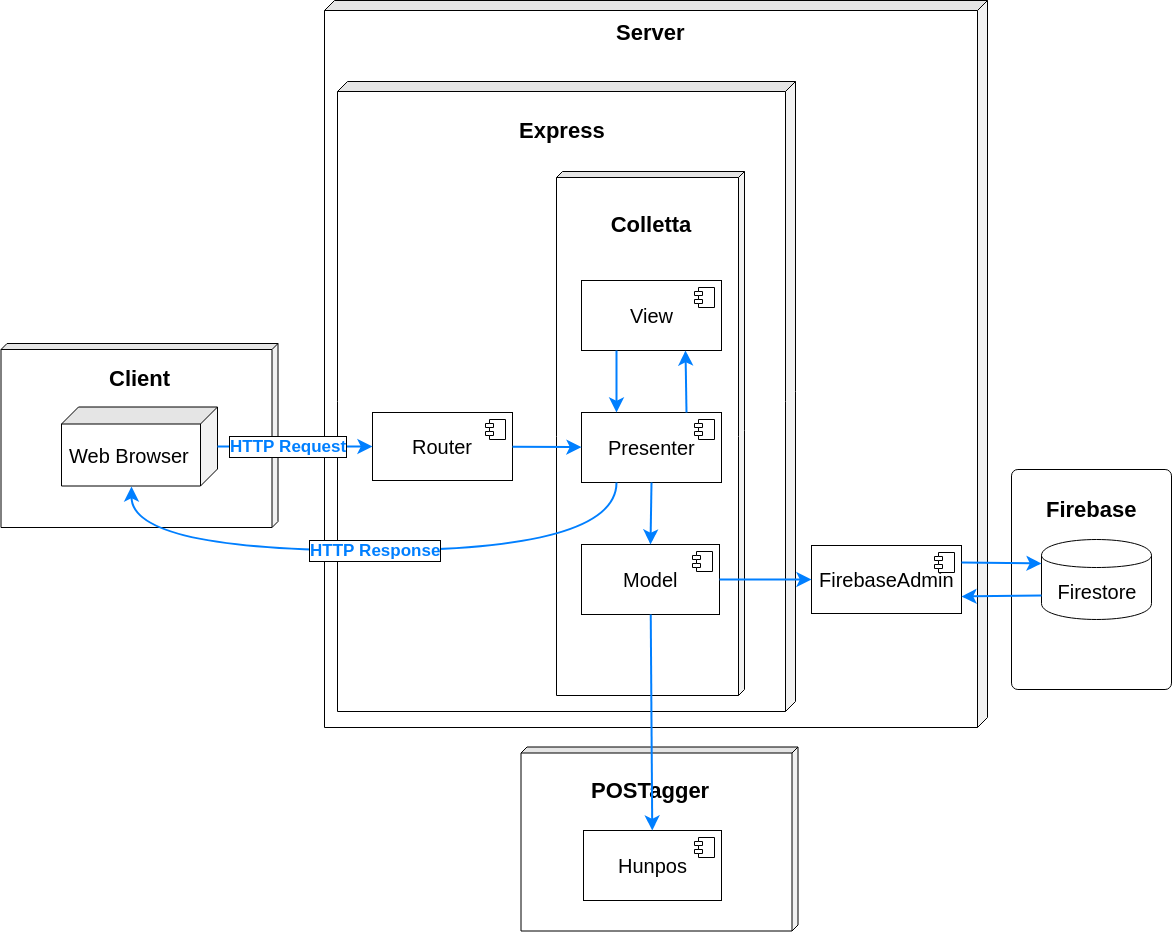
\includegraphics[scale=0.4]{images/architettura.png}
	\caption{Schema generale dell'applicazione}
\end{figure}

\paragraph*{Routing\\}
\noindent Il routing è realizzato dal framework Express e le richieste HTTP vengono smistate tra i vari presenter dell'applicazione, secondo il pattern Model-View-Presenter, ovvero:
\begin{enumerate}
	\item le routes inviano le richieste dell'utente che vengono realizzate da uno specifico presenter;
	\item i presenters operano sul modello, ottengono i dati necessari alla visualizzazione delle pagine e le costruiscono;
	\item le views sono passive e definiscono come sono costituite le varie pagine che verranno visualizzate dall'utente.
\end{enumerate}

\subparagraph*{Routes di visualizzazione}
\begin{itemize}
	\item \texttt{/home}: visualizza la vista principale dell'applicazione, con una barra di input di testo per lo svolgimento di un esercizio;
	\item \texttt{/profile}: visualizza il profilo dell'utente autenticato;
	\item \texttt{/exercise}: visualizza un form per lo svolgimento di un esercizio;
	\item \texttt{/exercise/insert}: visualizza un form per l'inserimento di un esercizio;
	\item \texttt{/registration}: visualizza un form per la registrazione alla piattaforma;
	\item \texttt{/class}:
	\item \texttt{/developer}:
	\item \texttt{/classes}:
	\item \texttt{/exercises}:
	\item \texttt{/exercise/search}:
	\item \texttt{/student/insert}:
	\item \texttt{/class/exercise/search}:
\end{itemize}

\subparagraph*{Routes di utilità}
\begin{itemize}
	\item \texttt{/checklogin}: permette di controllare l'identità di un utente che ha richiesto l'autenticazione;
	\item \texttt{/saveuser}: permette la scrittura delle credenziali di un utente nel database;
	\item \texttt{exercise/save}: permette la scrittura dei dati di un esercizio nel database;
	\item \texttt{/deletestudent}:
	\item \texttt{/deleteexercise}:
	\item \texttt{/addstudent}:
	\item \texttt{/addexercise}:
	\item \texttt{/checkdeveloper}:
	\item \texttt{/download}: ??? CHIEDERE A PERRY O GIAN
	\item \texttt{/download\%model}: ??? CHIEDERE A PERRY O GIAN
	\item \texttt{/exercise/update}:
	\item \texttt{/insertclass}:
	\item \texttt{/deleteclass}:
	\item \texttt{/update}:
	\item \texttt{/logout}:
	\item \texttt{/searchexercise}:
	\item \texttt{/searchstudent}:
	
	
\end{itemize}
\newpage

\subsection{Organizzazione della base informativa}
La base informativa è incentrata sui dati più importanti per la nostra applicazione, ovvero esercizi, classi e utenti. Ogni esercizio salvato nel database ha, inoltre, una o più soluzioni.

\begin{itemize}
	\item \texttt{Exercise}: ogni esercizio viene identificato da un codice e possiede una frase (univoca all'interno del database);
	\item \texttt{Class}: ogni classe viene identificato da un codice, possiede un nome (univoco) e dei riferimenti agli studenti, all'insegnante e agli esercizi ad esso assegnati;
	\item \texttt{User}: ogni utente viene identificata da un codice, possiede dei dati personali (come nome, cognome, città, scuola) e le credenziali di accesso; inoltre, se l'utente non è un insegnante il campo \texttt{teacher} contiene \texttt{-1}.
\end{itemize}

\begin{figure}[ht]
	\centering
	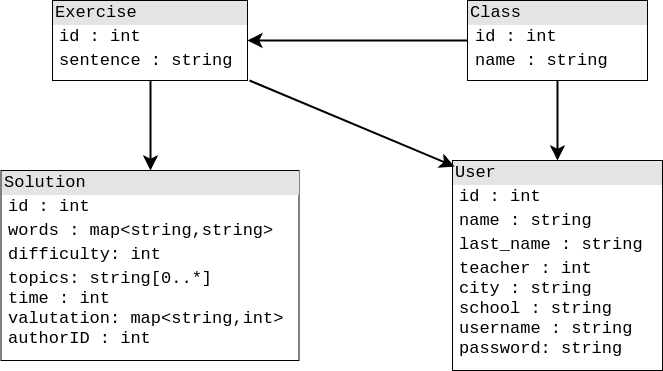
\includegraphics[scale=0.65]{images/database.png}
	\caption{Schema della base informativa}
\end{figure}
\newpage

\subsection{Organizzazione dei packages}
Più in dettaglio, abbiamo suddiviso ulteriormente il model in:
\begin{itemize}
	\item POSManager: parte dell'applicazione che si occupa dell'uso del software di apprendimento automatico;
	\item Data: l'insieme delle classi di business che permettono di svolgere le operazione di calcolo sui dati estratti dal database;
	\item Firebase: insieme di classi usate per l'utilizzo del database fornito da Firebase;
	\item Database: insieme di classi che utilizzano quelle definite dal pacchetto Firebase e che disaccoppiano l'applicazione dall'implementazione del database;
	\item Client: il cui scopo è esporre le funzionalità del model.
\end{itemize}
\begin{figure}[h]
	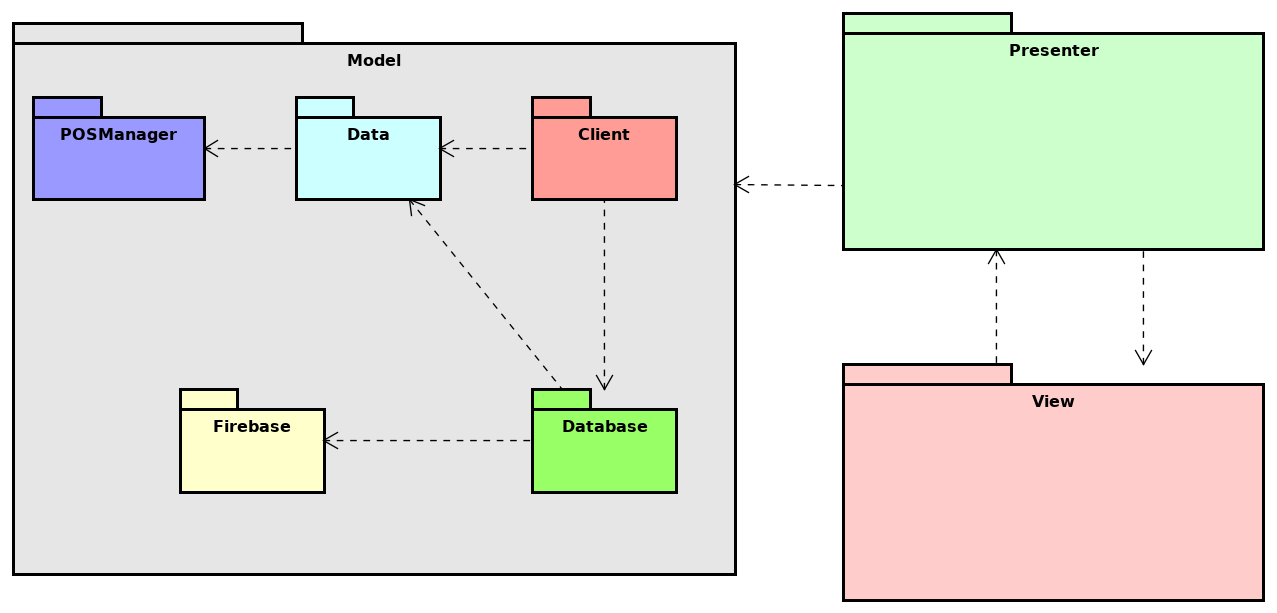
\includegraphics[scale=0.5]{images/package.png}
	\caption{Diagramma dei package}
\end{figure}
\newpage

\subsection{View}
Le viste sono organizzate seguendo una classe base che definisce la struttura di base di una qualsiasi pagina HTML dell'applicazione.
\begin{itemize}
	\item \texttt{DeveloperView}: la vista dedicata allo sviluppatore che necessita di consultare i dati contenuti nella piattaforma; 
	\item \texttt{ProfileView}: la vista dedicata alla visualizzazione del profilo personale e alle relative informazioni (ad esempio, la media degli esercizi per lo studente e il numero di esercizi assegnati per l'insegnante);
	\item \texttt{SearchView}: la vista dedicata alla visualizzazione delle pagine di ricerca della piattaforma;
	\item \texttt{ExerciseView}: la vista dedicata allo svolgimento e all'inserimento degli esercizi nella piattaforma.
\end{itemize}

\begin{figure}[h]
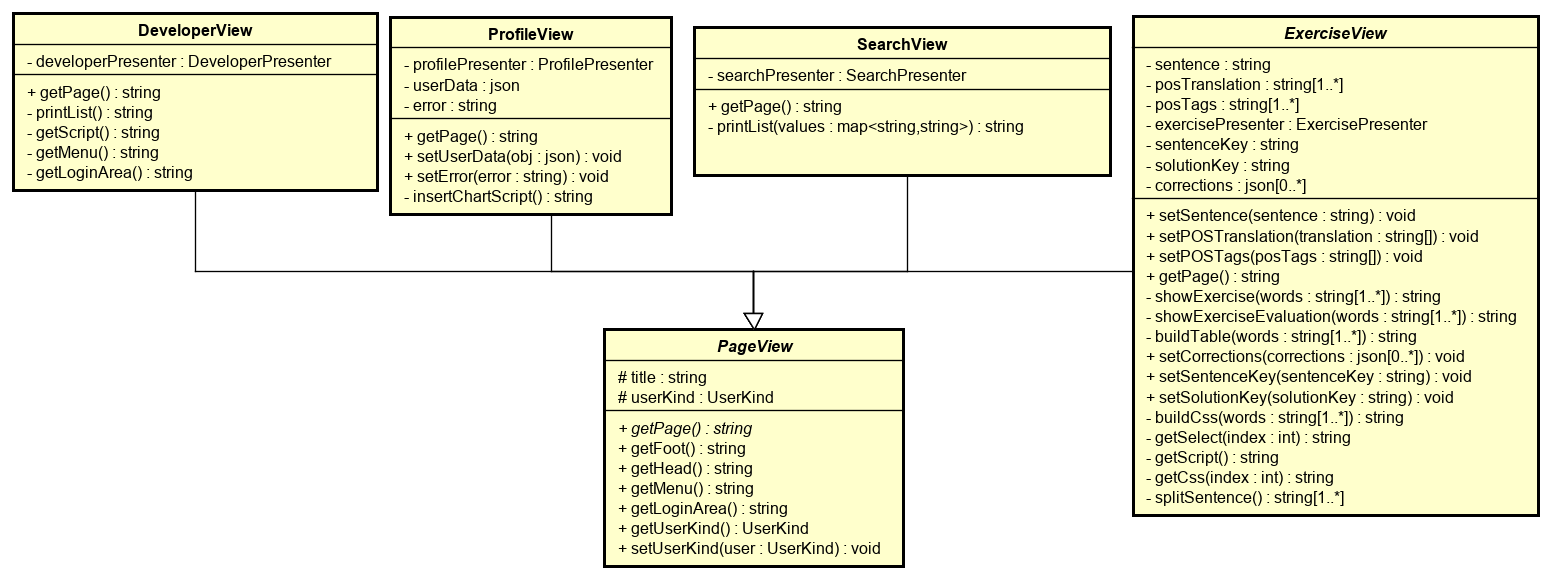
\includegraphics[scale=0.41]{images/View.png}
\caption{Diagramma delle classi di View}
\end{figure}

\newpage
\subsection{Presenter}
I presenter sono organizzati specularmente alle viste ed espongono le funzionalità necessarie per le pagine che gestiscono e definiscono la logica di controllo prelevando le informazioni dal modello. La classe base espone un metodo \texttt{update} che, usando Express, provoca l'aggiornamento della vista. Per offrire le funzionalità alle viste, i presenter hanno un riferimento alla vista e uno al modello dei dati.
\begin{itemize}
	\item \texttt{DeveloperPresenter}: il presenter dedicato alle funzionalità dello sviluppatore che necessita di consultare i dati ed il loro storico;
	\item \texttt{ProfilePresenter}: il presenter che si occupa di recuperare le informazioni legate a un singolo utente (ad esempio, la media degli esercizi per lo studente o il numero di esercizi assegnati per l'insegnante)
	\item \texttt{SearchPresenter}: il presenter dedicato alle funzionalità di ricerca nella piattaforma, come quella degli utenti e degli esercizi;
	\item \texttt{ExercisePresenter}: il presenter dedicato allo svolgimento e all'inserimento di un esercizio nella piattaforma.
\end{itemize}

\begin{figure}[h]
	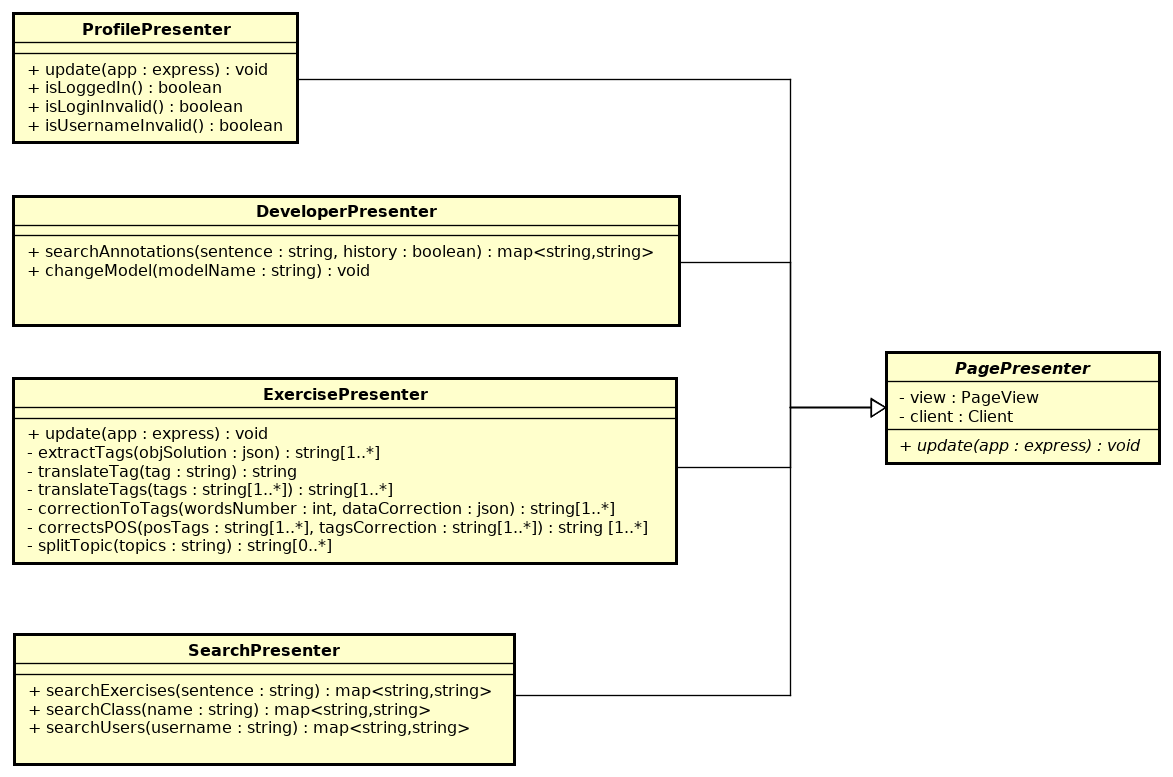
\includegraphics[scale=0.53]{images/Presenter.png}
	\caption{Diagramma delle classi del package Presenter}
\end{figure}

\newpage
\subsection{Model}
\subsubsection{Data}
\begin{figure}[ht]
	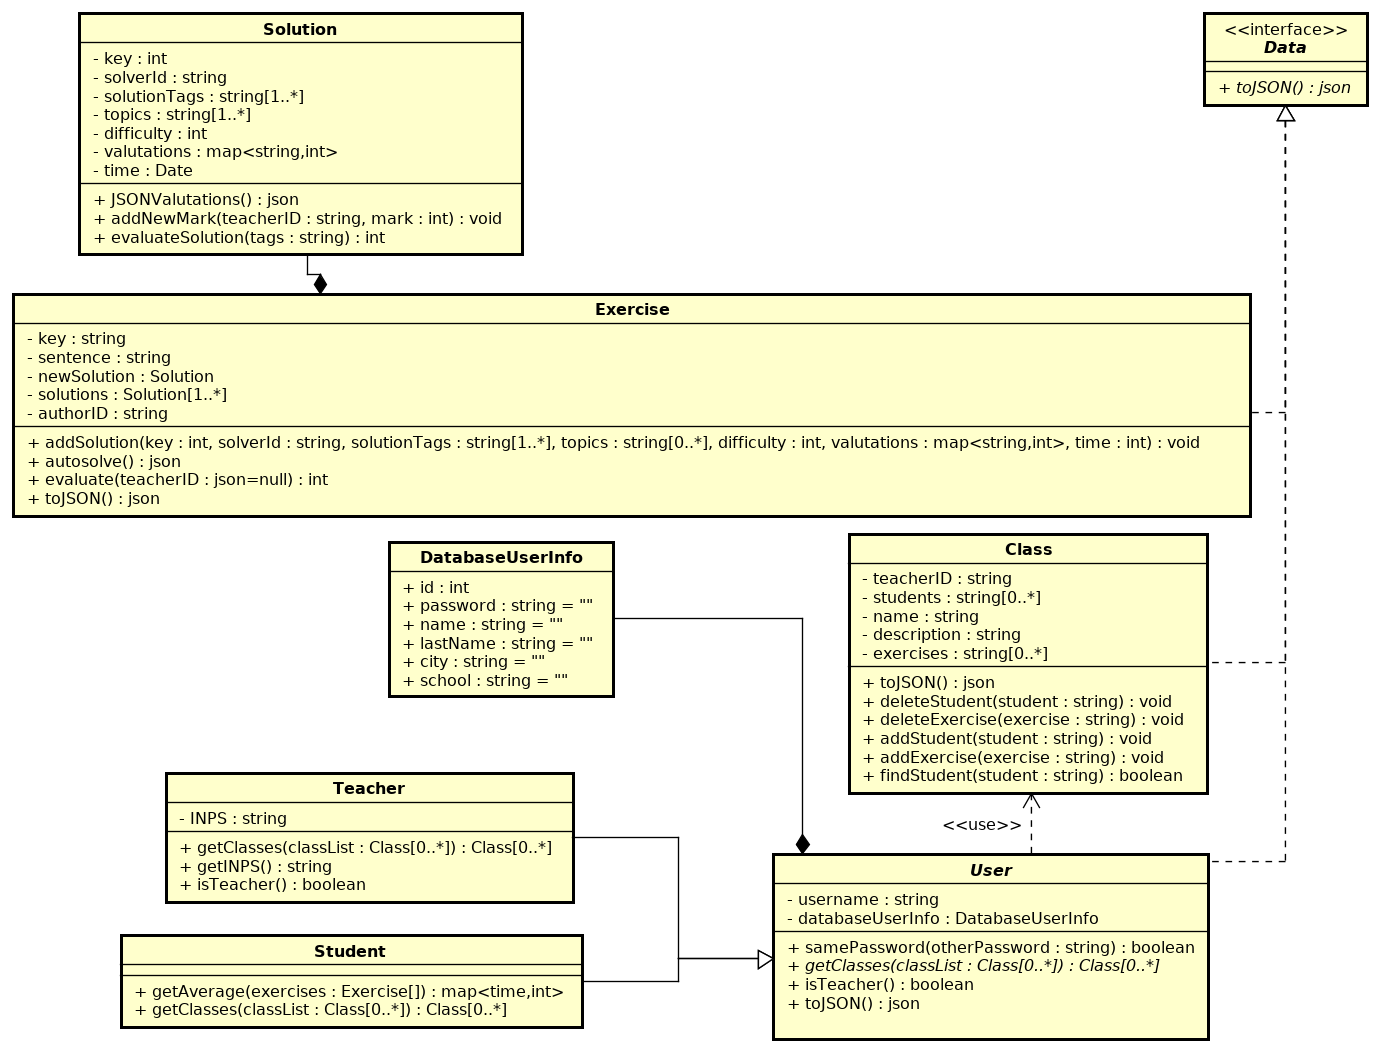
\includegraphics[scale=0.45]{images/Data.png}
	\caption{Diagramma delle classi del package Data}
\end{figure}

In Data si trovano tutte le classi di business dell'applicazione che permettono di calcolare valutazioni di esercizi, medie degli utenti e la risoluzione degli esercizi. Le classi rispecchiano la rappresentazione della base informativa.

\begin{itemize}
	\item \texttt{Data}: interfaccia che identifica tutti i dati rappresentati nel database;
	\item \texttt{Exercise}: modellazione di un esercizio presente nel database che espone le funzionalità necessarie allo svolgimento e alla valutazione di un esercizio da parte di un particolare insegnante;
	\item	\texttt{Solution}: modellazione di una soluzione di un esercizio che permette la valutazione della soluzione;
	\item \texttt{Class}: modellazione delle classi contenute nella piattaforma che mette in relazione studenti e insegnanti;
	\item \texttt{User}: modellazione di un utente qualsiasi registrato nella piattaforma che permette il calcolo delle informazioni correlate a tali utenti:
	\begin{itemize}
		\item \texttt{Teacher}: modellazione di un insegnante che permette il calcolo delle classi di cui esso è insegnante;
		\item \texttt{Student}: modellazione di uno studente che permette il calcolo dell'andamento della media delle valutazioni e delle classi a cui appartiene.
	\end{itemize}
\end{itemize}


\subsubsection{POSManager}
POSManager fornisce il modo di svolgere esercizi tramite il software di POS-tagging. Il pacchetto fornisce un'interfaccia che ogni software di questo tipo deve soddisfare, ovvero le operazioni di training e tagging e la capacità di restituire il risultato di quest'ultima operazione. In particolare, HunposManager è dotato di ulteriori funzioni che permettono la costruzione della soluzione. 

\begin{figure}[ht]
	\centering
	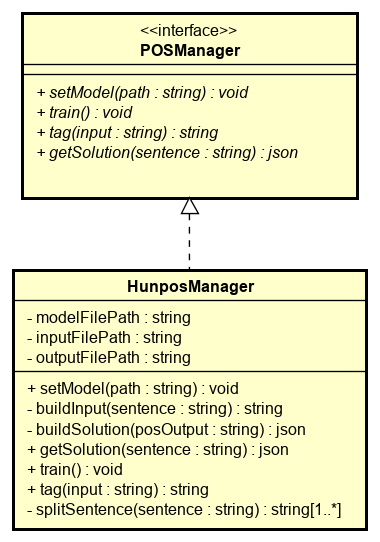
\includegraphics[scale=0.5]{images/POSManager.png}
	\caption{Diagramma delle classi del package POSManager}
\end{figure}
\newpage

\subsubsection{Database}
Database gestisce l'utilizzo del database tramite le classi DatabaseManager e derivate. La suddivisione rispecchia la rappresentazione dei dati all'interno della base di dati. In particolare:
\begin{itemize}
	\item \texttt{DatabaseExerciseManager}: permette le operazioni CRUD$^{*}$ e di ricerca degli esercizi;
	\item \texttt{DatabaseClassManager}: permette le operazioni CRUD e di ricerca delle classi;
	\item \texttt{DatabaseUserManager}: permette le operazioni CRUD e di ricerca degli User.
\end{itemize}
Questa gerarchia di classi agevola, in caso di ristrutturazione dell'applicazione, la sostituzione della base di dati dell'applicazione, semplicemente cambiando il riferimento al database. In questo caso, sarà necessario modificare il riferimento della classe al database. Tale modifica sarà però circoscritta a questa gerarchia di classi senza alcuna necessità di modificare le altre classi dell'applicazione.
\begin{figure}[h]
	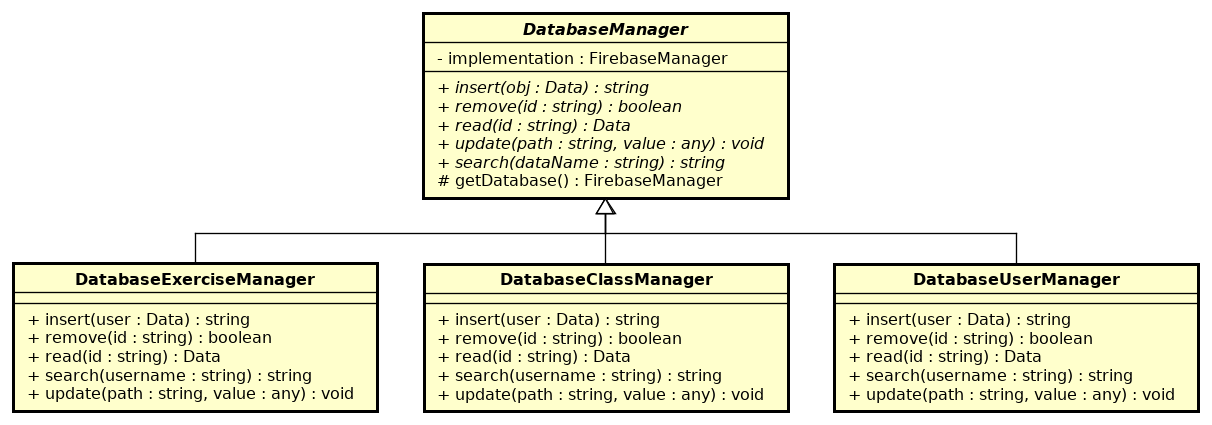
\includegraphics[scale=0.5]{images/DatabaseManager.png}
	\caption{Diagramma delle classi del package Database}
\end{figure}

\newpage
\subsubsection{Firebase}
Firebase rappresenta l'implementazione del database dell'applicazione e permette l'uso del database Firestore fornito da Firebase. In particolare:
\begin{itemize}
	\item \texttt{FirebaseExerciseManager}: permette le operazioni CRUD e di ricerca degli esercizi su Firestore;
	\item \texttt{FirebaseClassManager}: permette le operazioni CRUD e di ricerca delle classi su Firestore;
	\item \texttt{FirebaseUserManager}: permette le operazioni CRUD e di ricerca degli User su Firestore.
\end{itemize}

\begin{figure}[h]
	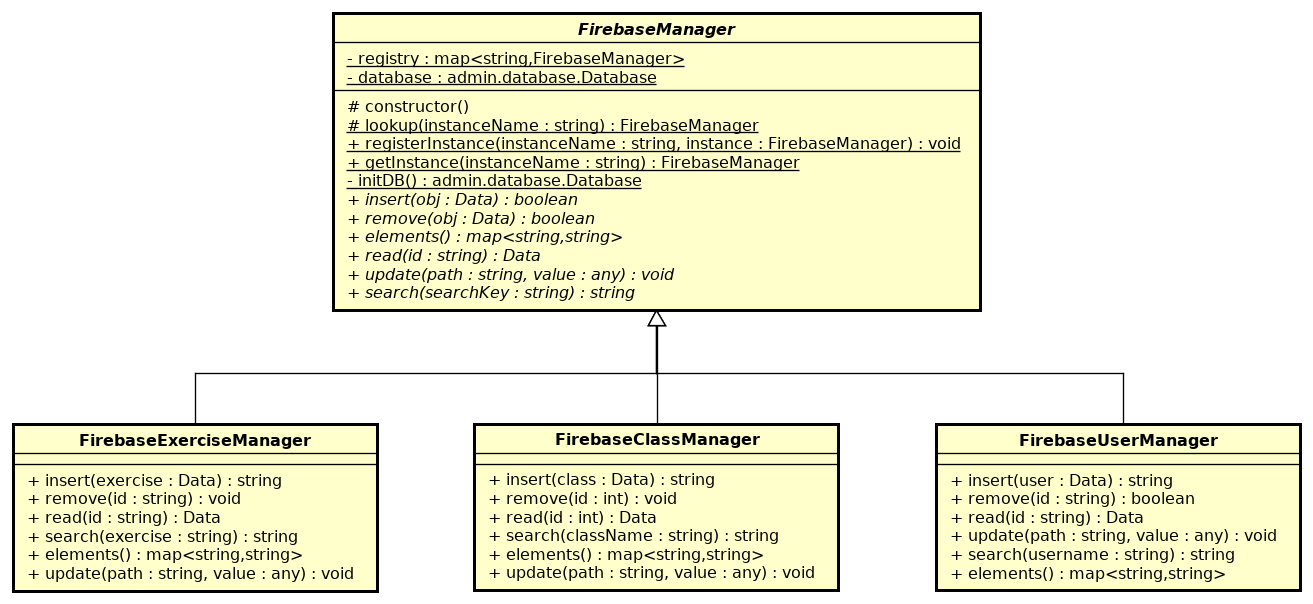
\includegraphics[scale=0.5]{images/FirebaseManager.png}
	\caption{Diagramma delle classi del package Firebase}
\end{figure}

\newpage
\subsubsection{Client}
Client è composto da diverse classi che espongono le varie funzionalità sul modello. In particolare, la classe \texttt{Client} è una composizione di funzionalità fornite da:
\begin{itemize}
	\item \texttt{ExerciseClient}: fornisce le funzionalità di inserimento, risoluzione e ricerca degli esercizi;
	\item \texttt{ClassClient}: fornisce le funzionalità di inserimento e recupero delle informazioni delle classi e l'assegnazione degli esercizi;
	\item \texttt{UserClient}: fornisce le funzionalità di inserimento e verifica dell'identità degli utenti.
\end{itemize}

\begin{figure}[ht]
	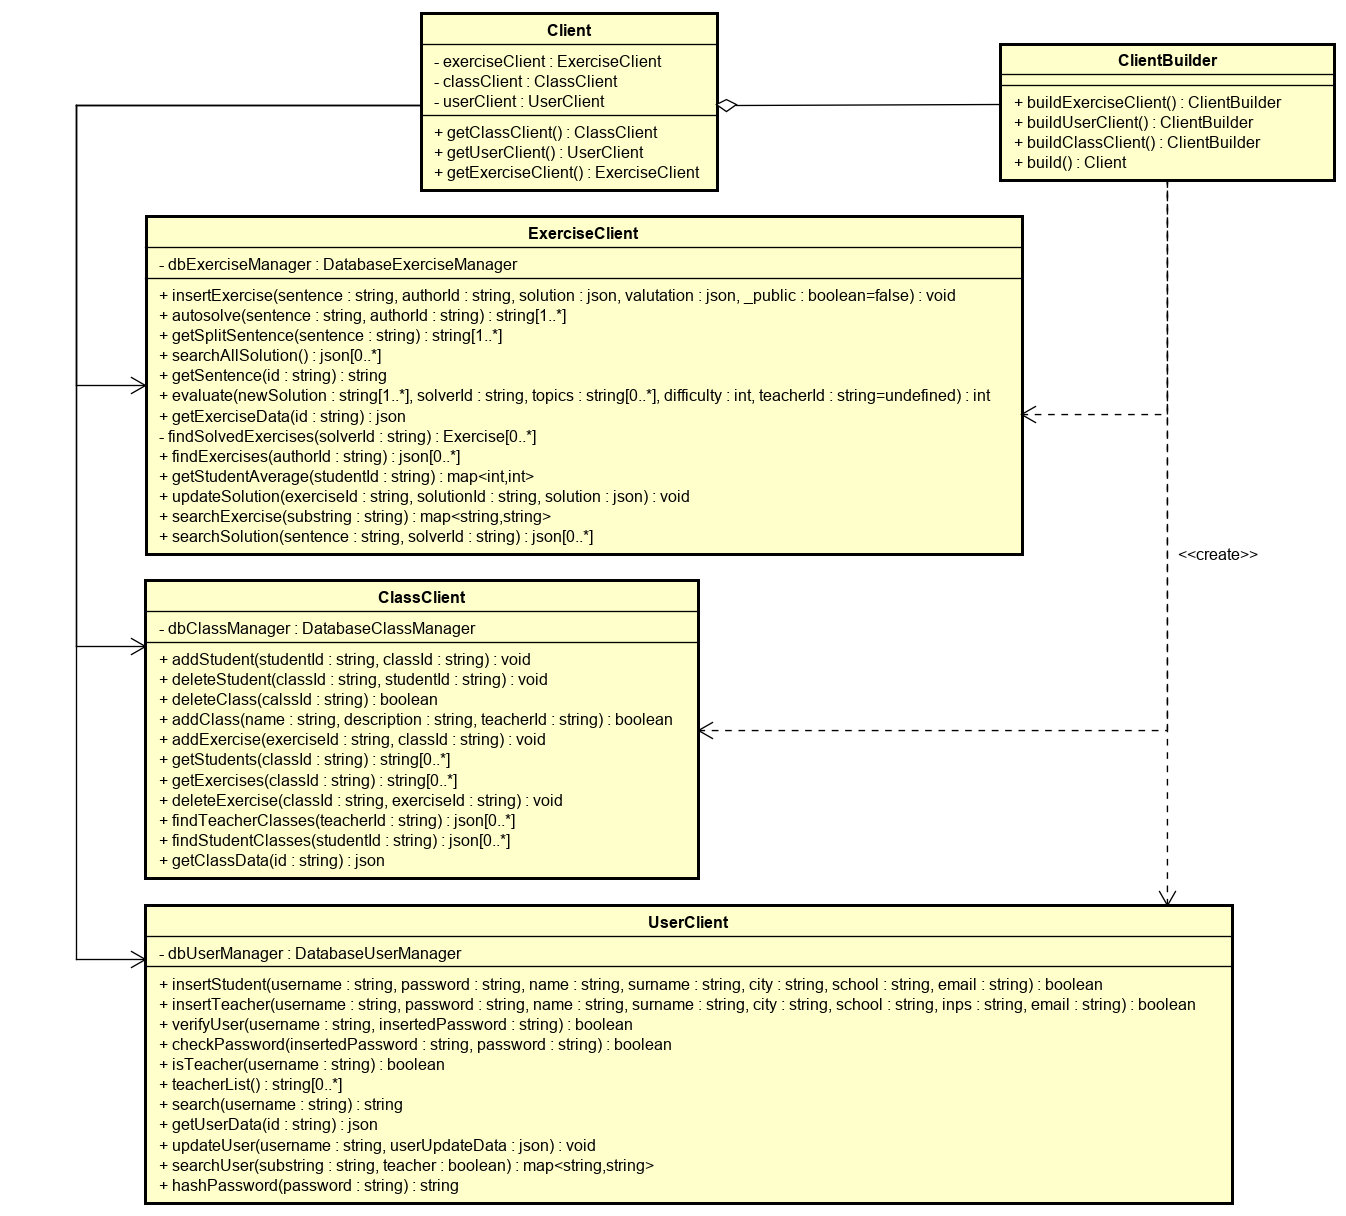
\includegraphics[scale=0.5]{images/Client.png}
	\caption{Diagramma delle classi del package Client}
\end{figure}


\newpage
	\newpage

	
		
\end{document}